% Created 2018-09-26 Wed 21:07
% Intended LaTeX compiler: pdflatex
\documentclass[journal=ancac3,manuscript=article,email=true,hyperref=true,keywords=false]{achemso}
\usepackage[utf8]{inputenc}
\usepackage{graphicx}
\usepackage{float}
\usepackage{xcolor}
\usepackage{amsmath}
\usepackage{amssymb}
\usepackage{lineno}
\usepackage{todonotes}
\usepackage{times}

\author{Tian Tian}
\affiliation{Institute for Chemical and Bioengineering, ETH Z{\"{u}}rich,  Vladimir Prelog Weg 1, CH-8093 Z{\"{u}}rich, Switzerland}
\altaffiliation{T. T. and D. S. contributed equally to this work}
\author{Declan Scullion}
\affiliation{School of Mathematics and Physics, Queen's University Belfast, BT7 1NN, United Kingdom}
\altaffiliation{T. T. and D. S. contributed equally to this work}
\author{Dale Hughes}
\affiliation{School of Mathematics and Physics, Queen's University Belfast, BT7 1NN, United Kingdom}
\author{Lu Hua Li}
\affiliation{Institute for Frontier Materials, Deakin University, Waurn Ponds, Victoria, Australia}
\author{Chih-Jen Shih}
\affiliation{Institute for Chemical and Bioengineering, ETH Z{\"{u}}rich,  Vladimir Prelog Weg 1, CH-8093 Z{\"{u}}rich, Switzerland}
\author{Jonathan Coleman}
\affiliation{School of Physics, Centre for Research on Adaptive Nanostructures and Nanodevices (CRANN) and Advanced Materials and BioEngineering Research (AMBER), Trinity College Dublin, Dublin 2, Ireland.}
\author{Manish Chhowalla}
\affiliation{Materials Science and Engineering, Rutgers University, 607 Taylor Road, Piscataway, New Jersey 08854, USA.}
\author{Elton J. G. Santos}
\email{e.santos@qub.ac.uk}
\affiliation{School of Mathematics and Physics, Queen's University Belfast, BT7 1NN, United Kingdom}
\date{}
\title{Unified Understanding of the Dielectric Nature of Two-Dimensional Materials}
\begin{document}

\newpage{}


\section{Introduction}
\label{sec:org2ea169d}

The central place of dielectric properties, especially the static
dielectric constant in material research
\cite{Dressel_2001_electrodynamics} drives the pursuit for a unified
model between the electronic and dielectric properties of materials.
In fact, some pioneering work\cite{Moss_1950_relation} discovered
relationships between the dielectric constant $\varepsilon$ and other
physical properties, in particular the band gap $E_{\mathrm{g}}$
(minimal optical transition energy) of bulk
semiconductors. Moss\cite{Moss_1950_relation,Moss_1985_n_Eg} showed
that $E_{\mathrm{g}}$ and $\varepsilon$ follow a semi-empirical
relationship, known as the Moss relation:
\begin{equation}
\label{eq:Moss-relations}
\varepsilon^{2} E_{\mathrm{g}} \approx 95\ \mathrm{eV}
\end{equation}
Other similar semi-empirical models for the relationship between
$\varepsilon$ and $E_{\mathrm{g}}$ of bulk semiconductors have also
been proposed
\cite{Ravindra_1979_eps_Eg,Ravindra_1980_model,Ravindra_2007_Eg_rev}. Despite
the minor difference between the formulae used, it is clear that there
exists certain general electronic relations in bulk
semiconductors. The existence of such general relationship is also of
high practical importance: it is generally more straightforward and
accurate to measure the band gap $E_{\mathrm{g}}$ than the static
dielectric constant $\varepsilon$, as the latter is strongly dependent
on several critical details on the sample measurements, such as
contamination, disorder, and model interpretation. With the Moss
relationship or other similar models, it is feasible to predict the
dielectric constant of a bulk semiconductor with a reasonable degree
of certainty.

While the relation between the electronic and dielectric properties
for bulk semiconductors are well-established, it is unknown if such
relation still exists in low-dimensional materials. For instance,
two-dimensional (2D) materials, the atomically-thin crystalline layers
\cite{Novoselov_2016}, are known to have distinct electronic
\cite{Mak_2010,Tran_2014} and dielectric properties
\cite{Keldysh_1979_eps_multi,Sharma_1985} compared with their bulk
counterparts, making the empirical relations of dielectric constant in
bulk materials, like the Moss relation invalid within the context of
2D materials. More critically, the static dielectric constant, a
quantity associated with the macroscopic dielectric property and
commonly obtained by theoretical calculations of 2D materials
\cite{Ramasubramaniam_2012,Wang_2016_Aip,Laturia_2018}, may not well
describe the microscopic and anisotropic dielectric nature of 2D
materials
\cite{Cudazzo_2010_screen2D,Cudazzo_2011_screening_2D}. Therefore, an
accurate description of the 2D dielectric nature is the prerequisite
for a 2D Moss-like relation. Here we show that instead of the
dielectric constant $\varepsilon$, the 2D polarizabilty $\alpha$
correctly captures the dielectric nature of a 2D material for both
in-plane and out-of-plane polarizations. Based on first principles
simulation of over 50 kinds \todo{some more?} of monolayer 2D
materials, we reveal the long-sought universal dielectric scale
relation in the 2D world: the in-plane polarizability
$\alpha^{\parallel}$ is inversely proportional to the minimal bandgap
$E_{\mathrm{g}}$, while the out-of-plane polarizability
$\alpha^{\perp}$ is closely related with the intrinsic thickness of 2D
materials. The anisotropy of the 2D polarizability is further
explained by a confined quantum model. The universal relations provide
quantitative prediction of the dielectric properties of 2D materials,
which leads to better design and understanding of electronic devices
based on 2D materials and their heterostructures. Furthermore, such
relations bridge the dielectric properties between the 2D materials
and their 3D counterparts, and ultimately pushes the boundary of the
understanding of electronic screening in both dimensions.

\section{Results}
\label{sec:org752ca78}

\subsection{Dielectric Nature of 2D Materials}
\label{sec:2d}

In persuit of the Moss-like relation of 2D materials, a accurate
description of the dielectric properties of 2D materials needs to be
established. One known issue is that the concept of macroscopic
dielectric constant is ill-defined for 2D materials
\cite{Cudazzo_2010_screen2D,Cudazzo_2011_screening_2D,Nazarov_2015_2D_3D}. As
shown in Figure \ref{fig-1}a \todo{I'll change upon your change of Fig
  1a}, in first principles calculations, an isolated 2D material is
placed at the xy-plane of a periodically repeating superlattice (SL)
with a length $L$ along the z-direction large enough to prevent the
interactions between periodic images. The macroscopic dielectric
tensor from the superlattice $\varepsilon_{\mathrm{SL}}$, from
fundamental electrostatics, is determined by the response of
volumetric dipole density $\boldsymbol{P}^{p}$, under small perturbative
external field $\boldsymbol{E}^{q}$, where $p$, $q$ are the
directions in $(x, y, z)$,such that:
\begin{subequations}
  \begin{eqnarray}
      \label{eq:def-eps-1}
    &\varepsilon^{p} &= \kappa^{pq} +
                                 {\displaystyle \frac{\partial \boldsymbol{P}^{p}}
                                 {\varepsilon_{0} \partial \boldsymbol{E}^{q}}} \\
          \label{eq:def-eps-2}
    &\boldsymbol{P}^{p} &=  {\displaystyle \frac{\boldsymbol{u}^{p}}{\Omega}}
                          = {\displaystyle \frac{{\displaystyle
          \int_{\mathrm{SL}} \rho(\boldsymbol{r}) \boldsymbol{r}^{p} d^{3}\boldsymbol{r}}}
                          {AL}}
  \end{eqnarray}
\end{subequations}
$\kappa$ is the dielectric tensor of the environment, $\boldsymbol{u}$
is the total dipole moments of the SL, $\rho$ is the spatial charge
density, $\Omega=AL$ is the volume of the SL, $A$ is the xy-plane area
of the SL and $\varepsilon_{0}$ is vacuum permittivity. For the
majority of 2D semiconductors, the off-diagonal elements of the
dielectric tensor ($p \neq q$) tend to be negligible.  Consider that
the 2D material is placed in vacuum, such that $\kappa^{pp} \equiv 1$
and $\kappa^{pq} \equiv 0$, we can distinguish two components of the
SL dielectric tensor, namely the in-plane
($\varepsilon_{\mathrm{SL}}^{\parallel}$) and out-of-plane
($\varepsilon_{\mathrm{SL}}^{\perp}$) dielectric constants, where
$\varepsilon_{\mathrm{SL}}^{\parallel} =
(\varepsilon_{\mathrm{SL}}^{xx} + \varepsilon_{\mathrm{SL}}^{yy})/2$
and
$\varepsilon_{\mathrm{SL}}^{\perp} = \varepsilon_{\mathrm{SL}}^{zz}$
\todo{geometry or numerical average?}. Due to the absence of bonding
along the z-direction, the induced charge density of a 2D material is
highly confined. Figure \ref{fig-1}a demonstrates the charge density
difference between zero and finite electric fields,
$\Delta \rho=\rho(\boldsymbol{E}) - \rho(\boldsymbol{E}=0)$ along the
z-axis for an isolated 2H-MoS$_{2}$ layer under
$|\boldsymbol{E}_{z}|=0.01 \mathrm{V\cdot \AA}^{-1}$, which only
extends to ~12 \AA{} along the z-direction inside the SL. When $L$ is
large enough that the induced dipoles from periodic images do not
overlap, the total dipole moments $\boldsymbol{u}$ of the SL in
Eq. \ref{eq:def-eps-2} is independent of $L$. As a consequence, we can
see from Eqs. \ref{eq:def-eps-1} and \ref{eq:def-eps-2}, that both
$\varepsilon^{\parallel}_{\mathrm{SL}}$ and
$\varepsilon^{\perp}_{\mathrm{SL}}$ depend on the SL length $L$. We
show this by plotting $\epsilon^{\parallel}_{\mathrm{SL}}$ and
$\epsilon^{\perp}_{\mathrm{SL}}$ as functions of $L$ for 2H-type group
6 transitional metal dichalcogenides (TMDCs, 2H-MX$_{2}$, where M=Mo,
W and X=S, Se, Te), in the top panels of Figure \ref{fig-1}b and
\ref{fig-1}c \todo{change order!}, respectively. We can also observe
that neither $\varepsilon^{\parallel}_{\mathrm{SL}}$ nor
$\varepsilon^{\perp}_{\mathrm{SL}}$ converges with the superlattice
length $L$ due to fact that the long-range Coulomb interaction could
not be completed screened, which is computationally unpractical
\cite{Hueser_2013_2Dvs3D}. The $L$-dependency of macroscopic
dielectric constant makes it erroneous to use
$\varepsilon_{\mathrm{SL}}$ to present the dielectric nature of a 2D
material. Therefore, we need to find a $L$-independent quantity to
present the intrinsic dielectric properties of the 2D materials. As
discussed previous, since the total dipole moments $\mathbf{u}$ remain
constant with $L$, we can define the surface or sheet polarization
density matrix $\boldsymbol{\mu}$, by multiplying
Eq. \ref{eq:def-eps-2} with $L$, that
$\boldsymbol{\mu}^{p} = \boldsymbol{P}_{p}L = \int_{\mathrm{SL}}
\rho(\boldsymbol{r}) \boldsymbol{r}_{p}d^{3} \boldsymbol{r}/A$,
independent of the superlattice size. Similar to the definition of
molecular polarizability \cite{Israelachvili_2011}, the sheet
polarization density $\boldsymbol{\mu}$ is associated with the 2D
polarizability tensor $\alpha$ through:
$\boldsymbol{\mu}^{p} = \sum_{q} \alpha^{pq}
\mathbf{E}_{\mathrm{loc}}^{q}$ \cite{T_bik_2004}, where
$E_{\mathrm{loc}}$ is the local electric field. In the in-plane
direction, the continuity of electric field gives
$\mathbf{E}^{\parallel}_{\mathrm{loc}}=\mathbf{E}^{\parallel}$
\cite{Markel_2016}. Perpendicular to the 2D plane, the dipole
screening yields
$\boldsymbol{E}_{\mathrm{loc}}^{\perp}=\boldsymbol{E}^{\perp}+\boldsymbol{\mu}^{\perp}/L$
\cite{Meyer_2001_dipole_slab,T_bik_2004}. Combining with
Eqs. \ref{eq:def-eps-1} and \ref{eq:def-eps-2}, we derive the
expressions for the in-plane and out-of-plane 2D polarizabilities,
$\alpha^{\parallel}$ and $\alpha^{\perp}$, respectively:
\begin{eqnarray}
  \label{eq:alpha-para-def}
  &\alpha^{\parallel} &= \varepsilon_{0}(\varepsilon_{\mathrm{SL}}^{\parallel} - 1)L\\
  \label{eq:alpha-perp-def}
    &\alpha^{\perp} &= \varepsilon_{0}\left(1 - {\displaystyle \frac{1}{\varepsilon_{\mathrm{SL}}^{\perp}}}\right)L
\end{eqnarray}
The bottom panels of Figure \ref{fig-1}b and \ref{fig-1}c show the
$\alpha^{\parallel}$ and $\alpha^{\perp}$ of the TMDCs as functions of
$L$, calculated using Eqs. \ref{eq:alpha-para-def} and
\ref{eq:alpha-perp-def}. We observe that both $\alpha^{\parallel}$ and
$\alpha^{\perp}$ remain almost constant when $L>$15 \AA{}. In
addition, by varying the value of $\alpha^{\parallel}$ and
$\alpha^{\perp}$, we can nicely reproduce the $L$-dependence of
$\varepsilon_{\mathrm{SL}}^{\parallel}$ and
$\varepsilon_{\mathrm{SL}}^{\perp}$, respectively (Figure \ref{fig-1}b
and \ref{fig-1}c insets). These findings indicate that the 2D
polarizability, instead of the dielectric constant, is the true
descriptor of the dielectric properties of 2D materials.

We note that the dielectric properties of 2D materials are also often
modeled using an effect medium approach, which treats the 2D material
as a slab with effective permittivity $\varepsilon_{\mathrm{2D}}$ and
thickness $\delta$
\cite{Sharma_1985,Cudazzo_2011_screening_2D,Matthes_2016,Trolle_2017_eps_subst,Laturia_2018}. Such
methods require \textit{a priori} determination of $\delta$, a
quantity with controversial definitions \cite{Mas_Ballest__2011}. In
such approaches, $\varepsilon_{\mathrm{2D}}$ and $\delta$ have to be
determined by fitting the $L$-dependent data of
$\varepsilon_{\mathrm{SL}}$, which is not only computational
expensive, but also fails to capture the anisotropy of the 2D
dielectric properties (details see Supplementary Section S1). On the
other hand, calculating 2D polarizabilities requires no knowledge of
$\delta$ (see Eqs. \ref{eq:alpha-para-def} and
\ref{eq:alpha-perp-def}), and correctly presents the anisotropy of 2D
dielectric nature that $\alpha^{\parallel} > \alpha^{\perp}$.  With
the polarizability as the true descriptor of 2D dielectric properties,
we will reveal the universal Moss-like relation of 2D materials.

\subsection{Universal Relations for 2D Polarizabilities}
\label{sec:first-principles}

In this letter, We study several types of 2D materials of different
electronic and optical properties, including transition metal
dichalcogenides (TMDCs, with the formula MX\(_{\text{2}}\), where M is
a metal in group 4, 6, 10 and X=O, S, Se, Te), metal monochalcogenides
(Ga$_{2}$S$_{2}$, Ga$_{2}$Se$_{2}$), cadmium halides (CdX$_2$, X=Cl,
I), hexagonal boron nitride (BN), graphene derivatives (fluorographene
(C$_{2}$F$_{2}$), graphane (C$_{2}$H$_{2}$)) and phosphorene (P$4$).
For the TMDCs, we consider 2 lattice phases, namely the 2H
(P\(\bar{6}\)m2 space group) and 1T (P3m1 space group).  The elements
involved in this study and the structures of the 2D materials are
shown in Figure \ref{fig-2}a and \ref{fig-2}b, respectively. The
static 2D polarizabilities are calculated from the static dielectric
response of the selected 2D materials using density functional theory
(DFT) with Heyd-Scuseria-Ernzerhof hybrid functionals (HSE06) in the
Vienna Ab Initio Simulation Package (VASP) including spin-orbit
coupling to avoid limitations on the description of band gaps and
dielectric functions. Further details for the first principle
calculations please refer to \textit{Methods}.

Figure \ref{fig-3}a shows the calculated $E_{\mathrm{g}}$ (blue dots)
and polarizabilities (bar plots) of all the 2D materials investigated,
covering a wide bandgap range of over 6 eV. The 2D polarizability
$\alpha $has the unit of Farad, and is more intuitive to be expressed
in the form $\alpha/(4 \pi \varepsilon_{0})$, which has the unit of
[Length] (similar to the molecular polarizability, which has the unit
of $4\pi \varepsilon_{0}\times$[Volume] \cite{Israelachvili_2011}). We
find that $\alpha^{\parallel}$ has a general descending trend when
$E_{\mathrm{g}}$ increases. On the other hand, no apparent trend
between $\alpha^{\perp}$ and $E_{\mathrm{g}}$ is observed (more
details see Supplementary Figure SXX \todo{TBD}). Recently, it is
found that the exciton binding energy $E_{\mathrm{b}}$ of 2D materials
exhibits universal linear relation with $E_{\mathrm{g}}$
\cite{Choi_linear_2015,Olsen_2016_hydrogen,Jiang_2017_Eg_Eb}. Combine
with the fact that the $E_{\mathrm{b}}$ is roughly inversely
proportional to $\alpha^{\parallel}$ \cite{Pulci_2014}, it is
reasonable to guess that a general linear correlation between
$E_{\mathrm{g}}$ and $1/\alpha^{\parallel}$ may exist for 2D
materials. Figure \ref{fig-3}c shows
$(4 \pi \varepsilon_{0})/\alpha^{\parallel}$ (in \AA{}) as a function
of $E_{\mathrm{g}}$ (in eV) for the 2D materials investigated, with a
linear regression slope of ~0.166 and $R^{2}$ of 0.84. We observe that
materials with lower $E_{\mathrm{g}}$ (<4 eV) generally lie close to
the regression line, while the deviation becomes greater for materials
with $E_{\mathrm{g}}>$4 eV, which has also been observed in the
$E_{\mathrm{b}}-E_{\mathrm{g}}$ relation of 2D materials
\cite{Olsen_2016_hydrogen,Jiang_2017_Eg_Eb}. We also observe that
$E_{\mathrm{g}}$ calculated on the HSE06 level shows better linear
correlation with $1/\alpha^{\parallel}$ compared with the bandgap
calculated using the Perdew–Burke–Ernzerhof (PBE) method (details see
Supplementary Information SXX \todo{TBD}). This can be explained by
the fact that the HSE06 hybrid functionals generally have a better
prediction for the bandgap of a material than the PBE method
\todo{some reference?}. It should be noted that although even more
accurate estimation of both $\varepsilon$ and $E_{\mathrm{g}}$ can be
achieved via many-body Green’s function method (GW) together with the
Bethe-Salpeter equation (BSE), the convergence of such method is known
to be highly affected by the dielectric screening of 2D materials
\cite{Hueser_2013_2Dvs3D} (see Supplementary Section SXX
\todo{}). Combining the accuracy, computational effort and
convergence, the choice of the HSE06 hybrid functional may be most
suitable to present the true relationship between $\alpha^{\parallel}$
and $E_{\mathrm{g}}$.

On the other hand, $\alpha^{\perp}$ is observed to be almost
independent of $E_{\mathrm{g}}$. Similar behavior is also observed for
molecular \cite{T_bik_2004} and carbon nanotube \cite{Benedict_1995}
systems when the polarizability is in the direct perpendicular to the
$\pi$ electron cloud. Meanwhile, while $\alpha^{\perp}$ is much
smaller than $\alpha^{\parallel}$, its magnitude can still span over 5
times among different materials, and generally larger for materials
with more atoms in the z-direction (such as Ga$_{2}$S$_{2}$) than
single-atom materials (such as BN). Starting from this observation and
the fact that 2D polarizability has unit of
$4\pi\epsilon\times$[Length], $\alpha^{\perp}$ may actually be related
to a characteristic length in the z-direction of a 2D material. Figure
\ref{fig-3}c shows $\alpha^{\perp}$ as a function of the covalent
thickness $\delta_{\mathrm{2D}}^{\mathrm{cov}}$. The covalent
thickness is defined as the longest distance in the z-direction
between any two atom nuclei plus their covalent radii, such that:
\begin{equation}
  \label{eq:cov-thick}
  \delta_{\mathrm{2D}}^{\mathrm{cov}} = \mathrm{max}(|z_{i} - z_{j}|
  + r_{i}^{\mathrm{cov}} + r_{j}^{\mathrm{cov}})
\end{equation}
where i, j are two atoms in the 2D material and $r^{\mathrm{cov}}_{i}$
is the covalent radius of atom i, as illustrated in Figure
\ref{fig-delta}. Surprisingly, $\alpha^{\perp}$ shows excellent linear
correlation with $\delta_{\mathrm{2D}}^{\mathrm{cov}}$, with
$R^{2}=0.98$, and a slope very close to $1/4\pi$. In other words, the
quantity $\alpha^{\perp}/\varepsilon_{0}$ can be regarded as the
long-sought-for characteristic thickness of 2D materials. In short, we
have revealed the 2D analog of the Moss relation for both polarization
direction: $\alpha^{\parallel}$ is inversely proportional to the
minimal bandgap $E_{\mathrm{g}}$, while $\alpha^{\perp}$ is the
characteristic thickness of the 2D material. The existence of such
universal scaling relation is confirmed by examining using the
recently-published C2DB database \cite{Haastrup_2018}, with the
dielectric properties of over 200 2D semiconductors calculated on the
PBE level (details see Supplementary Section SXX \todo{TBD}).  We have
further tested the potential relation between the 2D polarizabilities
with other physical quantities, including the effective carrier mass,
quantum capacitance and total atomic polarizabilities while no
apparent correlations are found (details see Supplementary Section SXX
\todo{note}). In the next section, we will show the theoretical
backgrounds of such universal relations of 2D polarizabilities.

\subsection{Theoretical Explanations}
\label{sec:theory}

Similar to the treatment of quantum wells (QW), the wavefunction of an
isolated 2D material $\psi(\mathbf{r})$ can be separated into the in-
and out-of-plane components \cite{davies_physics_1997}
$\psi^{\parallel}(\mathbf{\rho})$ and $\psi^{\perp}(z)$, such that
$\psi=\psi^{\parallel}\psi^{\perp}$, where $\mathbf{\rho}=(x, y)$ is
the in-plane coordinate. According to the Bloch theorem, the periodic
in-plane wavefunction can be further expressed as
$\psi^{\parallel}(\mathbf{\rho})=e^{ik\rho}u(\rho)$, where $k$ is the
in-plane wave vector and $u(\rho)$ is periodic function in the
xy-plane. According to the random phase approximation theory
\cite{Adler_1962}, $\varepsilon_{\mathrm{SL}}$ can be calculated by
taking the $\mathbf{q} \to 0$ and $\omega \to 0$ limits of the
non-interacting dielectric function $\varepsilon(\mathbf{q}, \omega)$,
where $\mathbf{q}$ is the momentum transfer and $\omega$ is the
frequency:
\begin{equation}
  \label{eq:RPA-eps2}
  \varepsilon_{\mathrm{SL}}
  = \varepsilon_{\mathrm{SL}}(\mathbf{q} \to 0)
  = 1 + \frac{2e^{2}}{\varepsilon_{0} |q|^{2} \Omega}
  \sum_{\mathrm{k, c, v}}
  \frac{|<\psi_{\mathrm{v}}(\mathbf{k})|e^{-i\mathbf{q}\mathbf{r}}|\psi_{\mathrm{c}}(\mathbf{k+q})>|^{2}}
  {E_{\mathrm{c}}(\mathbf{k+q}) - E_{\mathrm{v}}(\mathbf{k})}
  \left[f(\psi_{\mathrm{c}}) - f(\psi_{\mathrm{v}}))\right]
\end{equation}
where $e$ is the unit charge, c, v are the conduction and valence
bands, $f$ is the Fermi-Dirac distribution, $E$ is the eigenenergy of
individual bands, and $f$ is the Fermi-Dirac distribution. Taking the
limit that $L\to\infty$, when
$\varepsilon^{\perp}_{\mathrm{SL}} \approx 1$, we have
$1-1/\varepsilon^{\perp}_{\mathrm{SL}} \approx
(\varepsilon_{\mathrm{SL}}^{\perp} - 1)$. Therefore $\alpha^{\parallel}$ and $\alpha^{\perp}$ at 0 K can be unified by the same equation:
\begin{equation}
  \label{eq:alpha-RPA}
  \alpha = \frac{2e^{2}}{|q|^{2}A} \sum_{\mathrm{k,c,v}}
  \frac{|<\psi_{\mathrm{v}}(\mathbf{k})|e^{-i\mathbf{q}\mathbf{r}}|\psi_{\mathrm{c}}(\mathbf{k+q})>|^{2}}
  {E_{\mathrm{c}}(\mathbf{k+q}) - E_{\mathrm{v}}(\mathbf{k})}
\end{equation}
where the direction is determined by $\mathbf{q}$. For
$\alpha^{\parallel}$, $e^{-i\mathbf{qr}}$ is independent of
$z$. Further combining with the Bloch wave representation and the k-p
theory\cite{Jiang_2017_Eg_Eb}, we have:
\begin{equation}
  \label{eq:alpha_para_RPA}
  \alpha^{\parallel} = \frac{2e^{2}}
  {(2 \pi)^{2}} \int d^{2}\mathbf{k}
  \frac{|<u_{\mathrm{v}}(\mathbf{k})|\nabla|u_{\mathrm{v}}(k)>|^{2}}
  {E_{\mathrm{c}}(\mathbf{k}) - E_{\mathrm{v}}(\mathbf{k})}
\end{equation}
the final expression for Eq. \ref{eq:alpha_para_RPA} is shown to be
$\alpha^{\parallel} = N e^{2}/(2\pi E_{\mathrm{g}})$ by
Ref. \citenum{Jiang_2017_Eg_Eb}, where $N$ is degeneracy of bands
associated with the minimal bandgap. This explains the linear
correlation we observe between $1/\alpha^{\parallel}$ and
$E_{\mathrm{g}}$. When $\alpha^{\parallel}$ is measured in
$(4 \pi \varepsilon_{0})\cdot \mathrm{\AA}$ and $E_{\mathrm{g}}$
measured in eV, the linear regression slope in Figure \ref{fig-3}b is
predicted to be
$8\pi^{2}\varepsilon_{0} \mathrm{\AA}/(eN) \approx 0.436/N$. The
observed value of $\sim$0.166 corresponds to $N$ between 2 and 3,
which is reasonable for the 2D materials studied.

On the other hand, the $E_{\mathrm{g}}$ independence and correlation
with the covalent thickness of $\alpha^{\perp}$, can also be explained
using the same quantum framework. Generally speaking, $\psi^{\perp}$
follows the Hamiltonian in z-direction, such that:
\begin{equation}
  \label{eq:Hamil-z}
  \left[-\frac{\hbar^{2}}{2 m^{\perp}}\nabla^{2} + V(z)\right] \psi^{\perp}(z) = E \psi^{\perp}
\end{equation}
where $\hbar$ is the reduced Planck constant and $m^{\perp}$ is the
effective mass in the perpendicular direction. $V(z)$ is the potential
created by the 2D material, and confined within a region of length
$\delta$. For simplicity we use plane wave to model the in-plane
wavefunction, that
$\psi^{\parallel}(\mathbf{\rho}) \propto
e^{i\mathbf{k\rho}}$. Inserting into Eq. \ref{eq:alpha-RPA} and
perform the Taylor expansion of $e^{-i\mathbf{qr}}$, we can eliminate
the contribution from the in-plane
wavefunctions\cite{davies_physics_1997} and get:
\begin{equation}
  \label{eq:alpha_perp_RPA}
  \alpha^{\perp} = \frac{2e^{2}}{(2 \pi) ^{2}} \int d^{2}\mathbf{k}
  \sum_{\mathrm{c, v}}
  \frac{|<\psi_{\mathrm{v}}(\mathbf{k})|z|\psi_{\mathrm{c}}(\mathbf{k}>|^{2}}
  {E_{\mathrm{c}}(\mathbf{k}) - E_{\mathrm{v}}(\mathbf{k})}
\end{equation}
where the integration over $\mathbf{k}$ is done in the $k_{x}-k_{y}$
part of the Brillouin Zone. In a confined 1D system, the matrix
element
$<\psi_{\mathrm{v}}(\mathbf{k})|z|\psi_{\mathrm{c}}(\mathbf{k})>$ is
usually proportional to the length of confinement $\delta$, while the
eigenenergy difference $E_{\mathrm{c}}-E_{\mathrm{v}}$ is correlated
with $\delta^{-2}$, while independent of
$\mathbf{k}$\cite{Benedict_1995}. Therefore the integrated
$\alpha^{\perp}$ is also independent of the bandgap $E_{\mathrm{g}}$,
which would instead greatly influence $\alpha^{\parallel}$. Using a
simplified particle-in-box model, we evaluated the integration of
Eq. \ref{eq:alpha_perp_RPA} and show that $\alpha^{\parallel}$ is
related with the geometric parameter $\delta$ (details see Supplementary Section SXX \todo{add note}), the confinement of
electrons in the z-direction, which nicely explains our finding of
correlation between $\alpha^{\perp}$ and
$\delta^{\mathrm{cov}}_{\mathrm{2D}}$.

Based on unit analysis of the 2D polarizability, its in- and
out-of-plane components can be described as the characteristic
lengthes in both directions. In fact, such characteristic length is
just the dielectric screening length. The potential from a point
charge inside the 2D material generates an in-plane potential
$V(\rho)$ as function of distance $\rho$ from the point charge, in the
Keldysh form \cite{Keldysh_1979_eps_multi,Pulci_2014}:
\begin{equation}
  \label{eq:Keldysh}
  V(\rho) = \frac{e}{4 \alpha^{\parallel}}
  \left[H_{0}(\frac{2\varepsilon_{0}\rho}{\alpha^{\parallel}})
    - Y_{0}(2 \varepsilon_{0}\frac{\rho}{\alpha^{\parallel}})\right]
\end{equation}
The length $r^{\parallel}_{0} = \alpha^{\parallel}/(2\varepsilon_{0})$
determines the degree of in-plane dielectric screening: the charges
feel strong screening when $\rho/r^{\parallel}_{0} \ll 1$ while the
screening for $\rho/r^{\parallel}_{0} \gg 1$ reduces to the case of
vacuum. In other words, the quantity
$\alpha^{\parallel}/(2\varepsilon_{0})$ characterizes the radius of
localized in-plane screened potential. Combining with the result that
the thickness of 2D material is characterized by
$\alpha^{\perp}/\varepsilon_{0}$, we have drawn a generalized picture
of the dielectric nature of 2D materials via the 2D polarizability:
the dielectric screening of a point charge sitting in the middle of a
2D material can be viewed as an ellipsoid with the length of
principle axes to be $\alpha^{\parallel}/(2 \varepsilon_{0})$ and
$\alpha^{\perp}/(2 \varepsilon_{0})$, respectively. Beyond the
boundary the ellipsoid the dielectric screening gradually reduced to
the vacuum situation. Note such radius is not essentially the 2D
exciton radius, which is still related with the effective mass
\cite{Chernikov_2014_EB_MoS2_2D3D}. Nevertheless, with the universal
relation between $\alpha^{\parallel}-E_{\mathrm{g}}$ and
$\alpha^{\perp}-\delta_{\mathrm{2D}}^{\mathrm{cov}}$ for 2D materials,
we are able to quantitatively predict and design the dielectric nature
of a new 2D material by engineering the bandgap and geometry, which
can greatly enhance our understanding and application of 2D materials.



\subsection{Bridging the 2D and 3D Dielectric Properties}
\label{sec:2D-3D}

Apart from the universal relations we propose for the 2D materials, it
is also of high theoretical interest to model the transition of
dielectric properties from the 2D world to the 3D world. In other
words, can we describe the dielectric constants of a bulk layered
material from the polarizabilities of the monolayer (see Figure
\ref{fig-4}a)? The static dielectric constants
$\varepsilon_{\mathrm{bulk}}$ for a bulk material with equilibrium
interlayer distance $L_{\mathrm{bulk}}$, can be expressed using the
polarizabilities of the individual layers in the bulk material
$\alpha_{\mathrm{bulk}}$:
\begin{eqnarray}
  \label{eq:3D-para}
  &\varepsilon^{\parallel}_{\mathrm{bulk}} &= 1 + {\displaystyle \frac{\alpha_{\mathrm{bulk}}^{\parallel}}{\varepsilon_{0} L_{\mathrm{bulk}}}}\\
  \label{eq:3D-perp}
  &\varepsilon^{\perp}_{\mathrm{bulk}} &= \left(1 - \frac{\alpha_{\mathrm{bulk}}^{\perp}}{\varepsilon_{0} L_{\mathrm{bulk}}}\right)^{-1}
\end{eqnarray}
Note that $\alpha_{\mathrm{bulk}}$ may not essentially be the same as
$\alpha$ of isolated layer. Nevertheless we will first see how good
the predictions can be made when assuming
$\alpha_{\mathrm{bulk}}=\alpha$. Figure \ref{fig-4}b and \ref{fig-4}c
show the comparison between the
$\varepsilon_{\mathrm{bulk}}^{\parallel}$ and
$\varepsilon_{\mathrm{bulk}}^{\perp}$ from first principles DFT
calculations compared with the values predicted using Eqs
\ref{eq:3D-para} and \ref{eq:3D-perp}, respectively. We observe that
such approach provides good estimation of
$\varepsilon_{\mathrm{bulk}}^{\parallel}$, with the mean average error
(MAE) of 1.35. On the other hand, we observe the predicted values of
$\varepsilon_{\mathrm{bulk}}^{\perp}$ has good agreement with the DFT
values when $E_{\mathrm{g}}>4$ eV, while the deviation becomes larger
when $E_{\mathrm{g}}$ reduces. Such results means that the
$\alpha^{\parallel}$ in a bulk layered material can generally be
estimated from its 2D counterpart, while $\alpha^{\perp}$ differs from
the values of monolayer, as also observed in other studies
\cite{Andersen_2015_dielec_vdWH,Laturia_2018}. Two factors contribute
to the discrepancy: (i) the overlap between induced dipoles is larger
perpendicular to the plane than parallel to the plane, and (ii) the
interlayer coupling is larger for 2D materials with smaller
bandgap. If we have an accuracy approach to model
$\alpha_{\mathrm{bulk}}$ as function of $\alpha$ and the degree of
interlayer coupling $\eta$ \cite{Tkatchenko_2012}, the dielectric
transition from 2D to 3D would be smoothly described.

Next we will show how the relation between dielectric properties
transforms from 2D to 3D. Extend the approach for modeling
$\alpha^{\parallel}$ in Eq. \ref{eq:alpha_perp_RPA} to the bulk
material, and use the Bloch presentation for wavefunctions in all
dimensions, we get:
\begin{equation}
  \label{eq:alpha-Eg-3D}
  \varepsilon_{\mathrm{bulk}} = 1 + \frac{2e^{2}}{\varepsilon_{0}(2\pi)^{3}}\int d^{3}\mathbf{k}
  \frac{|<u_{\mathrm{v}}(\mathbf{k})|\nabla|u_{\mathrm{v}}(k)>|^{2}}
  {E_{\mathrm{c}}(\mathbf{k}) - E_{\mathrm{v}}(\mathbf{k})}
\end{equation}
Using a similar treatment for
$|<u_{\mathrm{v}}(\mathbf{k})|\nabla|u_{\mathrm{v}}(k)>|^{2}$ as in
Ref. \citenum{Jiang_2017_Eg_Eb} we end up with the relation
$\alpha_{\mathrm{bulk}} \propto 1/\sqrt{E_{\mathrm{g}}}$ (details see
Supplementary Section SXX \todo{note}), which recovers the Moss
relation under rigorous treatment \cite{Finkenrath_1988}. Therefore,
the universal $\alpha^{\perp}-E_{\mathrm{g}}$ relation is indeed the
Moss relation in 2D world, while the power law of $E_{\mathrm{g}}$ and
independence of effective mass is dominated by the confinement
perpendicular to the 2D plane.

Finally, we would like to comment on the generality of the dielectric
nature between the 2D and 3D worlds. As schematically shown in Figure
\ref{fig-2D-3D}, the physical quantities related to the dielectric
properties can be categorized into (i) strictly 2D (microscopic), (ii)
strictly 3D (macroscopic) and (iii) valid both 2D and 3D.  $\alpha$
and $\varepsilon$ are the starting point for the strictly 2D and 3D
quantities, which require distinct definitions when dimensionality
changes. Such quantities include (but not limited to):
\begin{enumerate}
\item The densities $n_{\mathrm{2D}}$ and $n_{\mathrm{3D}}$ for
  charge, polarization, electronic states, etc.
  
\item The plasma frequencies $\omega^{\mathrm{p}}_{\mathrm{2D}}$ and
  $\omega^{\mathrm{p}}_{\mathrm{2D}}$\cite{Nazarov_2015_2D_3D} (more
  details see Supplementary Section SXX \todo{TBD}).

\item The optical conductivity $\sigma_{\mathrm{2D}}$ and
  $\sigma_{\mathrm{3D}}$\cite{Bechstedt_2012,Matthes_2016}.
\end{enumerate}
These quantities have distinct units in both dimensions, and related
by $L$ (for density and optical conductivity) or $\sqrt{L}$ (for
plasma frequency), which requires prudent interpretation of
theoretical and experimental results. For instance, the experimentally
observed ``dielectric constant'' of monolayer 2D materials
\cite{Ning_2015,Li_2014,Yao_2014,Wu_2015} would be questionable
without considering the effect of mix ted medium. Instead, the 2D slab
polarizability, either transformed from the vacuum-containing
macroscopic dielectric constant, or predicted from the bandgap and
geometry as proposed here, will be a better descriptor for the true 2D
dielectric nature. On the other hand, there are also
dimension-independent quantities that valid for both 2D and 3D
systems, for instance the bandgap $E_{\mathrm{g}}$, exciton binding
energy $E_{\mathrm{b}}$, Bohr radius $r_{\mathrm{B}}$ of the exciton
as well as the Hamaker constant of van der Waals interaction
$A_{\mathrm{H}}$. All these quantities are well-defined and can be
measured in both dimensions, while their relation with the dielectric
property varies with dimensionality. The well-known examples are the
different Wannier-Mott laws for exciton binding energy
\cite{Olsen_2016_hydrogen}, the dielectric-bandgap relation
proposed here, and the distinct power laws for van der Waals
interactions \cite{Gobre_2013}. To get a accuracy description of
dielectric-related properties of the 2D materials and their
heterostructures, one has to distinguish between the 2D and 3D
properties, and choose a suitable relation with the
dimension-dependent and dimension-independent quantities.




\section{Conclusion}
\label{sec:org5fd1f1a}

To sum up, using first principles calculation for over 50 kinds of 2D
materials, we reveal the universal relation between the dielectric
nature of 2D materials and other physical quantities via the 2D
polarizability. The in-plane polarizability of a 2D material is found
to be inversely proportional to the minimal bandgap, while the
out-of-plane polarizability is the characteristic thickness of the 2D
material. Such universal scaling relation is explained by a quantum
mechanical model combining the polarizability in both directions. Our
universal scaling relation bridges the gap between 2D and 3D
dielectric properties with good accuracy of prediction.  Our numerical
findings and theoretical analysis pave the way to understand and
engineer the electronic and dielectric properties of a large library
of 2D materials for different technological applications in an
unified and unprecedented way.

\section{Theoretical Methods}
\label{sec:org8457dbb}

All results calculated for this paper were the result of \emph{ab
  initio} simulations carried out using plane-wave Density Functional
Theory (DFT) package VASP
\cite{Kresse_1993,Kresse_1996_1,Kresse_1996_2} using the Projector
Augmented Wave (PAW) approach with Kresse’s mainly GW
Pseudopotentials \cite{Kresse_1999_pseudopotentials}. Band gaps were
calculated using the Heyd-Scuseria-Ernzerhof hybrid functional (HSE06)
\cite{Heyd_2003,HSE_2006}, with Spin Orbit Coupling (SOC) explicitly
included. The geometries were converged both in cell parameters and
ionic positions, with forces below 0.04 eV/\AA. To ensure the accuracy
of dielectric property of monolayer, a vacuum spacing of $>$ 15 \AA is
used. A k-point grid of \(7\times7\times1\) was used to relax the
superlattice, with an initial relaxation carried out at the
Perdew-Burke-Ernzerhof
(PBE)\cite{Perdew_1996,Ernzerhof_1999,Paier_2005_PBE}
exchange-correlation functional level and a subsequent relaxation
carried out at HSE06 level, allowing both cell parameters and ionic
positions to relax each time. In VASP, the tag PREC=High was used,
giving a plane wave kinetic energy cutoff of 30\% greater than the
highest given in the pseudopotentials used in each material,
guaranteeing that absolute energies were converged to a few meV and
the stress tensor to within a few kBar.  Calculation of the
macroscopic ion-clamped dielectric tensor were carried out with an
18$\times$18$\times$1 k-grid and electric field strength of 0.001
eV/\AA. Bulk layered materials were constructed by relaxing the c-axis
length of corresponding monolayer material with the interlayer van der
Waals (vdW) interactions calculated by non-local vdW correlation
functional\cite{Lee_2010_vdFD2}. The dielectric properties of bulk
layered materials were calculated at PBE level with
18$\times$18$\times$6 k-grid with same parameter as for monolayer.



\bibliography{ref}

% \section{Figures}
\label{sec:org34cbe74}
\begin{figure}[htbp]
\centering
\includegraphics[width=0.90\linewidth]{img/fig1.pdf}
\caption{\label{fig-1} The macroscopic dielectric constant and
  microscopic polarizability of a 2D material. \textbf{a}. Left: 2D
  material in a superlattice with length $L$ in the z-direction. The
  periodic images of the 2D material are shown below and above the
  superlattice. Right: simplied presentation of the dielectric
  constants $\varepsilon_{\mathrm{SL}}^{\parallel}$ and
  $\varepsilon_{\mathrm{SL}}^{\perp}$ of the superlattice as a
  combined effect of the 2D polarizabilities $\alpha^{\parallel}$ and
  $\alpha^{\perp}$ and the vacuum. \textbf{b}. Change of spatial
  charge density $\Delta \rho(z)$ in the z-direction for a layer of
  2H-MoS$_{2}$ under external eletric field of 0.01 V/\AA{}. The green
  and red regions represent negative and positive induced charges,
  respectively. \textbf{c}. $\varepsilon^{\parallel}_{\mathrm{SL}}$
  (left) and $\alpha_{\mathrm{SL}}^{\parallel}$ (right) as functions
  of $L$ for a 2H-MoS$_{2}$
  layer. \textbf{d}. $\varepsilon^{\perp}_{\mathrm{SL}}$ (left) and
  $\alpha_{\mathrm{SL}}^{\perp}$ (right) as functions of $L$ for a
  2H-MoS$_{2}$ layer. The polarizabilities in \textbf{c} and
  \textbf{d} are constant when $L>$15 \AA{}.}
\end{figure}

\begin{figure}[htbp]
\centering
\includegraphics[width=0.8\linewidth]{./img/fig2.pdf}
\caption{\label{fig-2} The 2D materials investigated. \textbf{a}. The
  elements that involved in this study. \textbf{b} 3D structures of
  the 2D materials investigated in this study.}
\end{figure}

\begin{figure}[htbp]
\centering
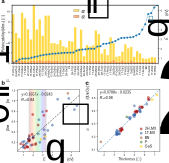
\includegraphics[width=0.95\linewidth]{./img/fig3.pdf}
\caption{\label{fig-3} The universal scaling relation of the
  dielectric nature of 2D materials. \textbf{a}. $\alpha^{\parallel}$,
  $\alpha^{\perp}$ (bar plots) and $E_{\mathrm{g}}$ (blue dots) for
  all the 2D materials studied.  $\alpha^{\parallel}$ is observed to
  descend with increasing $E_{\mathrm{g}}$, while no apparent relation
  between $\alpha^{\perp}$ and $E_{\mathrm{g}}$ is
  observed. \textbf{b}. $(4\pi \varepsilon_{0})/\alpha^{\parallel}$
  (in \AA{}) as a function of $E_{\mathrm{g}}$, showing a linear
  correlation between each other. The energy range of visible light is
  shown in the
  background. \textbf{c}. $\alpha^{\perp}/(4\pi\varepsilon_{0})$ (in
  \AA{}) as a function of the covalent thickness, showing a perfect
  linear relation with slope very close to $1/4\pi$. The materials in
  \textbf{b} and \textbf{c} are grouped by their prototyes, including
  1T-TMDCs and cadmium halide (1T-MX$_{2}$), 2H-TMDCs (2H-MX$_{2}$),
  boron nitride (BN), phosphorene (P), monochalcogenides (GaS) and
  graphene derivatives (CH).}
\end{figure}

\begin{figure}[htbp]
\centering
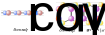
\includegraphics[width=0.5\linewidth]{img/fig-delta.pdf}
\caption{\label{fig-delta} Scheme for the determination of the
  covalent thickness of one-atom-thick (left) and few-atom-thick
  (right) 2D materials.}
\end{figure}

\begin{figure}[htbp]
\centering
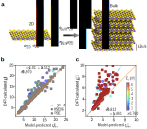
\includegraphics[width=\linewidth]{./img/fig4.pdf}
\caption{\label{fig-4} Transition of dielectric properties from 2D to
  3D systems. \textbf{a}. Scheme for the 2D-3D transition. $\alpha$ in
  the 2D material is essentially equivalent to $\varepsilon$ in its
  bulk counterpart. \textbf{b}
  $\varepsilon_{\mathrm{bulk}}^{\parallel}$ calculated from DFT
  (y-axis) compared with the predicted value from 2D
  $\alpha^{\parallel}$ (x-axis), showing good correlation. \textbf{c}
  $\varepsilon_{\mathrm{bulk}}^{\perp}$ calculated from DFT (y-axis)
  compared with the predicted value from 2D $\alpha^{\parallel}$
  (x-axis). The predicted value is in good aggreement with the DFT
  calculation when $E_{\mathrm{g}}>4$ eV, due to minimal interlayer
  coupling. }
\end{figure}

\begin{figure}[htbp]
\centering
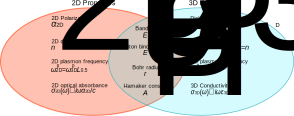
\includegraphics[width=0.75\linewidth]{img/fig-2D-vs-3D.pdf}
\caption{\label{fig-2D-3D} Dielectric-related physical quantities in
  both 2D (red circle) and 3D (cyan circle) systems. The
  dimension-dependent quantities can be related with $\alpha$ and
  $\varepsilon$, respectively. The intersection between the circles
  present the quantities are well-defined in both dimensions, but may have a
  different scaling relation with others quantities.}
\end{figure}
\end{document}